% Abhinav Kumar, MSU, 2020
% Use \command{}word for joining \xspace ending command and another word

%===============================================================================
% Colors
%===============================================================================
\definecolor{my_blue}{rgb}{0.2, 0.6, 1}  % dodgerblue
\definecolor{my_magenta}{rgb}{1.0, 0.2, 0.6} % triadic to dodgerblue
\definecolor{my_yellow}{rgb}{1.0, 0.8, 0.2} % triadic to magenta
\definecolor{my_green}{rgb}{0.0, 0.9, 0.24}
\definecolor{my_green_2}{rgb}{0.0, 0.4, 0.0}

% Seaborn colors
% colors_temp = sns.color_palette("magma", 10)
% sns[1] {0.2, 0.06, 0.40}
% sns[2] {0.34, 0.08, 0.49}
% sns[3] {0.49, 0.14, 0.51}
% sns[5] {0.78, 0.24, 0.45}
% sns[6] {0.91, 0.33, 0.38}
% \definecolor{sns_blue}{rgb}{0.2, 0.06, 0.40}
% \definecolor{sns_violet}{rgb}{0.34, 0.08, 0.49}
% \definecolor{sns_orange}{rgb}{0.91, 0.33, 0.38}
% colors_temp = sns.color_palette("magma", 20)
% sns[3]  {0.21, 0.06, 0.42}
% sns[6]  {0.45, 0.12, 0.51}
% sns[10] {0.75, 0.22, 0.46}
% sns[19] {0.99, 0.91, 0.66}
\definecolor{sns_blue}{rgb}{0.21, 0.06, 0.42}
\definecolor{sns_violet}{rgb}{0.45, 0.12, 0.51}
\definecolor{sns_orange}{rgb}{0.75, 0.22, 0.46}
\definecolor{sns_yellow}{rgb}{0.99, 0.91, 0.66}

%Citation color
\definecolor{white}{rgb}{1.0, 1.0, 1.0}
\definecolor{darkGreen}{rgb}{0.01, 0.8, 0.24}%{0.31, 0.94, 0.3}%{0.09,0.88,0.00}{0.29, 0.83, 0.38}
\definecolor{darkGreen2}{rgb}{0.22,0.42, 0.33}
\definecolor{darkGreen3}{rgb}{0.20,0.66, 0.33}
\definecolor{cvprblue}{rgb}{0.21,0.49,0.74}
\definecolor{LightCyan}{rgb}{0.88,1,1}
\definecolor{lightgreen}{HTML}{90EE90}
\definecolor{new_green}{rgb}{0.75,0.97,0.44}
\definecolor{Gray}{gray}{0.95}
\definecolor{lightgray}{rgb}{0.96, 0.96, 0.96}

\definecolor{set1_cyan}{rgb}{0.23, 0.87, 1.0}
\definecolor{building}{rgb}{0.2, 0.33, 0.33}

\definecolor{my_violet}{rgb}{0.79, 0.40, 1} %{0.73,0.62,0.91}
\definecolor{my_yellow_2}{rgb}{0.9, 0.8, 0.54}
\definecolor{my_red}{rgb}{1,0,0}
\definecolor{my_purple}{rgb}{0.27,0.8, 0.8}
\definecolor{my_orange}{rgb}{1.0,0.6,0.35}
\definecolor{my_golden}{rgb}{1.0, 0.75, 0.0}
\colorlet{my_gray}{gray!12}

\definecolor{projectionColor}{rgb}{0.2, 0.6, 1}
\definecolor{rayColor}{rgb}{0.0,0.0,0.0}
\definecolor{axisColor}{rgb}{0.0, 0.0, 0.0}
\colorlet{projectionBorderShade}{rayColor!100}
\colorlet{projectionFillShade}{projectionColor!20}
\colorlet{rayShade}{my_yellow}
\colorlet{axisShade}{axisColor!20}
\colorlet{axisShadeDark}{axisColor!100}

\definecolor{backward_color}{rgb}{1.0, 0.6, 0.2}
\definecolor{forward_color}{rgb}{0.2, 1.0, 0.6}

% Table row Colors
\definecolor{gain}{HTML}{34a853}
\definecolor{lost}{HTML}{ea4335}

\colorlet{proposedShade}{darkGreen}
\colorlet{vanillaShade}{red!90}

\colorlet{theme_color}{sns_orange}%my_yellow
\colorlet{theme_color_light}{sns_yellow!25}

% Scale qualitative figures by this fraction
\newcommand{\figureScaleFraction}{0.9}
\newcommand{\waymoFigureScaleFraction}{0.61}

%===============================================================================
% Text
%===============================================================================
% No indent heading
\newcommand{\noIndentHeading}[1]{\noindent\textbf{#1}}

% Textual Comments
\newcommand{\question}[1]{\noindent\fontseries{sb}\textbf{#1}}
\definecolor{XLcolor}{rgb}{0.858, 0.188, 0.478}
\newcommand{\XL}[1]{{\color{XLcolor}{\textbf{XL}: #1}  }}  % Donot use \textcolor. It breaks for line-breaks.
\newcommand{\abhinav}{{\color{blue}{Abhinav}  }}
\newcommand{\shengjie}{{\color{orange}{Shengjie}}}
\newcommand{\YG}{\textcolor{blue}}
\newcommand{\CCtext}[1]{{\color{my_blue}{#1}}}
\newcommand{\futureWrite}[1]{{\color{red}{WRITE: #1}  }}

\newcommand{\green}[1]{\scriptsize\textcolor{ForestGreen}{#1}}
\newcommand{\red}[1]{{\color{red}#1}}
\newcommand{\todo}[1]{{\color{red}#1}}
\newcommand{\TODO}[1]{\textbf{\color{red}[TODO: #1]}}
\newcommand\colCancel[2][red]{\renewcommand\CancelColor{\color{#1}}\cancel{#2}}

% Latin abbreviations
%\newcommand{\eg}{\textit{e.g.}\xspace}
\newcommand{\forExample}{\textit{e.g.}\xspace}
\newcommand{\thatIs}{\textit{i.e.}\xspace}
\newcommand{\etcetera}{\textit{etc.}\xspace}
\newcommand{\argmax}{\operatornamewithlimits{argmax}}
% \newcommand{\wrt}{\textit{wrt}\xspace}
%\newcommand{\etal}{\textit{et~al.}\xspace}

\newcommand{\filledCircle}{\tikz\draw[black,fill=black] (0,0) circle (.7ex);}
\newcommand{\semiCircle}{\tikz\fill[black] (90:.7ex) -- (-90:.7ex) arc (-90:90:.7ex) -- cycle;}

% Tick and cross for present and absent
\newcommand{\cmark}{\checkmark}%\ding{51}}%
\newcommand{\xmark}{\ding{53}}
\newcommand{\autoBraces}[1]{\left(#1\right)}

%===============================================================================
% Mathematical Notations
%===============================================================================
\newcommand{\bigO}[1]{\mathcal{O}\left(#1\right)}
\newcommand{\clip}[1]{\left\lfloor#1\right\rceil}
\newcommand{\numberElem}[1]{\left|#1\right|}
\newcommand{\elementMul}{\!\odot} %\circ
\newcommand{\linfinity}{\ell_\infty}
\newcommand{\identity}{{\bf{I}}}
\newcommand{\tr}{^{\!\top}}
\newcommand{\invtr}{^{\text{-}\!\top}}
\DeclareMathOperator{\sign}{sgn}

%===============================================================================
% Tables
%===============================================================================
% Scale tables by this fraction
\newcommand{\scaleFraction}{0.9}

% Table rules
\newcommand{\myTopRule}{\Xhline{2\arrayrulewidth}}
\newcommand{\myMidRule}{\Xhline{1.5\arrayrulewidth}}

\newcolumntype{t}{!{\vrule width 1.5\arrayrulewidth}}
\newcolumntype{m}{!{\vrule width 2.5\arrayrulewidth}}
\newcolumntype{a}{>{\columncolor{theme_color_light}}l}
\newcolumntype{b}{>{\columncolor{theme_color_light}}c}

\newcommand{\CYMyFix}{\cellcolor{theme_color_light}}
\newcommand\scalemath[2]{\scalebox{#1}{\mbox{\ensuremath{\displaystyle #2}}}}

% Cell Cyan
\colorlet{cyan_highlight}{my_blue!85}
\newcommand{\CCFix}{\cellcolor{cyan_highlight}}
% Cell Green
\colorlet{darkGreen_highlight}{darkGreen!75}
\newcommand{\CGFix}{\cellcolor{darkGreen_highlight}}
% Cell Orange
\colorlet{my_magenta_highlight}{my_magenta!50}
\newcommand{\COFix}{\cellcolor{my_magenta_highlight}}
% Cell Yellow
\colorlet{my_yellow_highlight}{my_yellow!55}
\newcommand{\CYFix}{\cellcolor{my_yellow_highlight}}

% Fancy set of arrows
\providecommand\rightarrowRHD{\relbar\joinrel\mathrel\RHD}
\providecommand\rightarrowrhd{\relbar\joR101inrel\mathrel\rhd}
\providecommand\longrightarrowRHD{\relbar\joinrel\relbar\joinrel\mathrel\RHD}
\providecommand\longrightarrowrhd{\relbar\joinrel\relbar\joinrel\mathrel\rhd}

\newcommand{\uparrowRHD}  {\rotatebox[origin=c]{90}{$\rightarrowRHD$}}
\newcommand{\downarrowRHD}{\rotatebox[origin=c]{270}{$\rightarrowRHD$}}
% up and down arros for showing higher/lower the better
\newcommand{\uparrowRHDSmall}  {\raisebox{0.05\normalbaselineskip}{\scalebox{0.7}{\uparrowRHD}}}   %$\uparrow$
\newcommand{\downarrowRHDSmall}{\raisebox{0.07\normalbaselineskip}{\scalebox{0.7}{\downarrowRHD}}} %$\downarrow$

%===============================================================================
% Object Detection
%===============================================================================
\newcommand{\monoThreeD}{Mono3D\xspace}
\newcommand{\monoDE}{MonoDE\xspace}

\newcommand{\oneD}{$1$D\xspace}
\newcommand{\twoD}{$2$D\xspace}
\newcommand{\threeD}{$3$D\xspace}
\newcommand{\fourD}{$4$D\xspace}
\newcommand{\fiveD}{$5$D\xspace}
\newcommand{\sixD}{$6$D\xspace}
\newcommand{\twoDMath}{2\text{D}\xspace}
\newcommand{\threeDMath}{3\text{D}\xspace}
\newcommand{\iou}{IoU\xspace}
\newcommand{\iouTwoD}{IoU$_{2\text{D}}$\xspace}
\newcommand{\iouThreeD}{IoU$_{3\text{D}}$\xspace}
\newcommand{\iouThreeDMath}{\text{\iou}_{3\text{D}}\xspace}
\newcommand{\lidar}{LiDAR\xspace}
\newcommand{\lidars}{LiDARs\xspace}
\newcommand{\radar}{radar\xspace}
\newcommand{\Radar}{Radar\xspace}
\newcommand{\giouTwoD}{g\iouTwoD}
\newcommand{\giouThreeD}{g\iouThreeD}
\newcommand{\vol}{V}
\newcommand{\bev}{BEV\xspace}

% Backbone
\newcommand{\dla}{DLA-34\xspace}
\newcommand{\dlaThirtyFour}{DLA-34\xspace}
\newcommand{\dlaOneZeroTwo}{DLA-102\xspace}
\newcommand{\dlaOneSixNine}{DLA-169\xspace}
\newcommand{\denseNetOneTwoOne}{DenseNet-121\xspace}
\newcommand{\resNetEighteen}{ResNet-18\xspace}
\newcommand{\resNetFifty}{ResNet-50\xspace}
\newcommand{\resNetOneHundredOne}{ResNet-101\xspace}
\newcommand{\rsuNet}{RSUNet\xspace}
\newcommand{\vovNet}{V2-99\xspace}
\newcommand{\efficientDet}{EfficientDet\xspace}
\newcommand{\pretrain}{pretrain\xspace}
\newcommand{\bigRes}{320\!\times\!1024}
\newcommand{\smallRes}{192\!\times\!680}

% Datasets
\newcommand{\kitti}{KITTI\xspace}
\newcommand{\nuscenes}{nuScenes\xspace}
\newcommand{\waymo}{Waymo\xspace}
\newcommand{\waymoOpen}{Waymo Open\xspace}
\newcommand{\imageNet}{ImageNet\xspace}
\newcommand{\nyuDepth}{NYU-Depth-v2\xspace}
\newcommand{\valOne}{Val 1\xspace}
\newcommand{\valTwo}{Val 2\xspace}
\newcommand{\val}{Val\xspace}
\newcommand{\valSmall}{val}
\newcommand{\frontal}{frontal\xspace}
\newcommand{\advWeather}{Adverse Weather\xspace}
\newcommand{\advWeatherShort}{Adv. Weather\xspace}
\newcommand{\ithaca}{Ithaca-365\xspace}
\newcommand{\argoverseTwo}{Argoverse 2\xspace}
\newcommand{\scannet}{ScanNet\xspace}
\newcommand{\rugd}{RUGD\xspace}
\newcommand{\kittiThreeSixty}{KITTI-360\xspace}
\newcommand{\kittiThreeSixtyPanoptic}{\kittiThreeSixty PanopticBEV\xspace}
\newcommand{\semanticKITTI}{Semantic KITTI\xspace}
\newcommand{\carla}{CARLA\xspace}
\newcommand{\ddad}{DDAD\xspace}

% Loss 
\newcommand{\loss}{\mathcal{L}}
\newcommand{\lossBefore}{\loss_{before}}
\newcommand{\lossAfter}{\loss_{after}}
\newcommand{\lossWeigh}{\lambda}
\newcommand{\aploss}{\ap-Loss}
\newcommand{\imageWise}{Imagewise}
\newcommand{\lOne}{\loss_1}
\newcommand{\lTwo}{\loss_2}
\newcommand{\smoothLOne}{\text{Smooth}~\lOne}
\newcommand{\lIoU}{\loss_{iou}}
\newcommand{\lDice}{\loss_{dice}}
\newcommand{\dice}{dice\xspace}
\newcommand{\Dice}{Dice\xspace}
\newcommand{\lSmooth}{\loss_{smooth}}
\newcommand{\size}{\text{size}}
\newcommand{\offset}{\text{offset}}
\newcommand{\heatmap}{\text{heatmap}}
\newcommand{\class}{{class}}
\newcommand{\weightSeg}{\lambda_{seg}}

% Metric
\newcommand{\MAP}{mAP\xspace}
\newcommand{\MAPLarge}{AP$_{Lrg}$\xspace}
\newcommand{\MAPCar}{AP$_{Car}$\xspace}
\newcommand{\MAPSmall}{AP$_{Sml}$\xspace}
\newcommand{\ap}{AP\xspace}
\newcommand{\apMath}{\text{\ap}}
\newcommand{\apThreeD}{$\apMath_{3\text{D}}$\xspace}
\newcommand{\apHThreeD}{APH$_{3\text{D}}$\xspace}
\newcommand{\apThreeDForty}{\ap$_{3\text{D}|R_{40}}$\xspace}
\newcommand{\apBevForty}{\ap$_{\text{BEV}|R_{40}}$\xspace}
\newcommand{\apTwoD}{\ap$_{2\text{D}}$\xspace}
\newcommand{\apTwoDForty}{\ap$_{2\text{D}|R_{40}}$\xspace}
\newcommand{\mate}{mATE\xspace}
\newcommand{\mase}{mASE\xspace}
\newcommand{\maoe}{mAOE\xspace}
\newcommand{\mave}{mAVE\xspace}
\newcommand{\maae}{mAAE\xspace}
\newcommand{\NDS}{NDS\xspace}

\newcommand{\levelOne}{Level\_1\xspace}
\newcommand{\levelTwo}{Level\_2\xspace}
\newcommand{\bracketPercentage}{[\%]}
\newcommand{\imageOnly}{image-only\xspace}
\newcommand{\apThreeDFifty}{\ap$_{\!3\text{D}\!}$ 50\xspace}
\newcommand{\apThreeDTwentyFive}{\ap$_{\!3\text{D}\!}$ 25\xspace}

\newcommand{\absRel}{Abs Rel\xspace}
\newcommand{\sqRel}{Sq Rel\xspace}
\newcommand{\rmse}{RMSE\xspace}
\newcommand{\rmseLog}{RMSE log\xspace}
\newcommand{\logTen}{log$_{10}$\xspace}
\newcommand{\siLog}{SI\textsubscript{log}\xspace}
\newcommand{\aOne}{a_1\xspace}
\newcommand{\aTwo}{a_2\xspace}
\newcommand{\aThree}{a_3\xspace}
\newcommand{\aTau}{a_\tau}

\newcommand{\meanFor}{M$_\text{For}$}
\newcommand{\meanEleven}{M$_\text{All}$}

% Ranking
\newcommand{\first}[1]{$\textcolor{sns_blue}{\mathbf{#1}}$}
\newcommand{\second}[1]{$\textcolor{sns_orange}{\mathbf{#1}}$}
\newcommand{\firstKey}[1]{\textcolor{sns_blue}{\textbf{#1}}}
\newcommand{\secondKey}[1]{\textcolor{sns_orange}{\textbf{#1}}}
\newcommand{\sota}{SoTA\xspace}
\newcommand{\best}[1]{$\textcolor{sns_blue}{\mathbf{#1}}$}
\newcommand{\bestKey}[1]{\textcolor{sns_blue}{\textbf{#1}}}
\newcommand{\gain}[1]{\textcolor{gain}{#1}}
\newcommand{\lost}[1]{\textcolor{lost}{#1}}
\newcommand{\good}[2]{{$#1$} {({\gain{\textbf{+}$\mathbf{#2}$}})}}
\newcommand{\bad}[2]{{$#1$} {({\lost{--$#2$}})}}
\newcommand{\arxiv}{ArXiv\xspace}
\newcommand{\mySign}{\!+\!}
\newcommand{\mathDash}{$-$}

\def\relicon{\resizebox{.009\textwidth}{!}{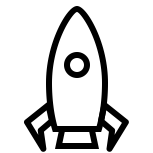
\includegraphics{images/1410037-200.png}}}
\newcommand{\released}{$\!^{\relicon}$}
\newcommand{\retrained}{$\!^\dagger$}
\newcommand{\reimplemented}{$\!^*$}
\newcommand{\cbgs}{$\!^{\mathsection}$}
\newcommand{\future}{$\!^{\tiny{\fullmoon}\hspace{-0.03cm}\tiny{\newmoon}}$}%{$\!{\circ}$}

% Previous Mono3D Methods
\newcommand{\mthreeDRPN}{M3D-RPN\xspace}
\newcommand{\kinematicImage}{Kinematic (Image)\xspace}
\newcommand{\kinematicVideo}{Kinematic (Video)\xspace}
\newcommand{\groomedNMS}{GrooMeD-NMS\xspace}
\newcommand{\monoDISMulti}{MonoDIS-M\xspace}
\newcommand{\gupNet}{GUP Net\xspace}
\newcommand{\deviant}{DEVIANT\xspace}
\newcommand{\pseudoLidar}{Pseudo-{\lidar}\xspace}
\newcommand{\ddThreeD}{DD3D\xspace}
\newcommand{\ddmp}{DDMP-3D\xspace}
\newcommand{\caddn}{CaDDN\xspace}
\newcommand{\patchNet}{PatchNet\xspace}
\newcommand{\monodtr}{MonoDTR\xspace}
\newcommand{\monorun}{MonoRUn\xspace}
\newcommand{\monodle}{MonoDLE\xspace}
\newcommand{\monodetr}{MonoDETR\xspace}
\newcommand{\monopair}{MonoPair\xspace}
\newcommand{\dFourLCN}{D4LCN\xspace}
\newcommand{\detrThreeD}{DETR3D\xspace}
\newcommand{\fcosThreeD}{FCOS3D\xspace}
\newcommand{\pgd}{PGD\xspace}
\newcommand{\petr}{PETR\xspace}
\newcommand{\petrVTwo}{PETRv2\xspace}
\newcommand{\bevFormer}{BEVFormer\xspace}
\newcommand{\polarFormer}{PolarFormer\xspace}
\newcommand{\bevDepth}{BEVDepth\xspace}
\newcommand{\bevStereo}{BEVStereo\xspace}
\newcommand{\bevDetFourD}{BEVDet4D\xspace}
\newcommand{\beVerse}{BEVerse\xspace}
\newcommand{\beVerseTiny}{BEVerse-T\xspace}
\newcommand{\beVerseSmall}{BEVerse-S\xspace}
\newcommand{\orBoxNet}{Box Net\xspace}
\newcommand{\uvtr}{UVTR\xspace}
\newcommand{\veDet}{VEDet\xspace}
\newcommand{\cape}{CAPE\xspace}
\newcommand{\xThreeKDAll}{X3KD$_{\text{all}}$\xspace}
\newcommand{\frustumFormer}{FrustumFormer\xspace}
\newcommand{\threeDPPE}{3DPPE\xspace}
\newcommand{\hop}{HoP\xspace}
\newcommand{\parametricBEV}{ParametricBEV\xspace}
\newcommand{\sparseBEV}{SparseBEV\xspace}
\newcommand{\saBEV}{SA-BEV\xspace}
\newcommand{\fbBEV}{FB-BEV\xspace}
\newcommand{\streamPETR}{StreamPETR\xspace}
\newcommand{\bevDetFourDHoP}{BEVDet4D+HoP\xspace}
\newcommand{\beVerseWithMethod}{BEVerse+SeaBird\xspace}
\newcommand{\beVerseTinyWithMethod}{BEVerse-T+SeaBird\xspace}
\newcommand{\beVerseSmallWithMethod}{BEVerse-S+SeaBird\xspace}
\newcommand{\bevDetFourDHoPWithMethod}{BEVDet4D+HoP+SeaBird\xspace}
\newcommand{\hopWithMethod}{HoP+SeaBird\xspace}
\newcommand{\stxd}{STXD\xspace}
\newcommand{\cubeRCNN}{Cube R-CNN\xspace}

% Previous BEV Segmentation Papers
\newcommand{\imageToMaps}{I2M\xspace}
\newcommand{\imageToMapsLong}{Image2Maps\xspace}
\newcommand{\imageToMapsWithMethod}{I2M+SeaBird\xspace}
\newcommand{\panopticBEV}{PBEV\xspace}
\newcommand{\panopticBEVLong}{PanopticBEV\xspace}
\newcommand{\panopticBEVWithMethod}{PBEV+SeaBird\xspace}

% Previous Radar Image Detection Papers
\newcommand{\centerFusion}{CenterFusion\xspace}
\newcommand{\grifNet}{GRIF Net\xspace}
\newcommand{\contFusion}{Cont Fusion\xspace}
\newcommand{\simpleBEV}{Simple-BEV\xspace}
\newcommand{\craft}{CRAFT\xspace}
\newcommand{\cramNet}{CramNet\xspace}
\newcommand{\radiant}{RADIANT\xspace}

% Previous Lidar Detection Papers
\newcommand{\lidarBoxNet}{L-BoxNet\xspace}
\newcommand{\voteNet}{L-VoteNet\xspace}

% Previous Denoising Papers
\newcommand{\mirNet}{MIRNet-v2\xspace}

% Previous MonoDepth Papers
\newcommand{\monoDepthTwo}{MonoDepth2\xspace}
\newcommand{\depthHints}{DepthHints\xspace}
\newcommand{\edgeDepth}{EdgeDepth\xspace}
\newcommand{\epcDepth}{EPCDepth\xspace}
\newcommand{\idisc}{iDisc\xspace}
\newcommand{\zoeDepth}{ZoeDepth\xspace}

% SLAM Papers
\newcommand{\slam}{SLAM\xspace}
\newcommand{\dynamicSLAM}{Dynamic \slam}
\newcommand{\timelineMarker}{$\CIRCLE$}
\newcommand{\selfMotion}{self-motion\xspace}
\newcommand{\SelfMotion}{Self-motion\xspace}
\newcommand{\SelfMotionCaps}{Self-Motion\xspace}
\newcommand{\objectMotion}{object motion\xspace}
\newcommand{\ObjectMotionCaps}{Object-Motion\xspace}
\newcommand{\task}{Task\xspace}
\newcommand{\taskAb}{T\xspace}
\newcommand{\subTask}{subtask\xspace}

% NeRF Papers
\newcommand{\nerf}{NeRF\xspace}
\newcommand{\nerfs}{NeRFs\xspace}
\newcommand{\autoRF}{AutoRF\xspace}
\newcommand{\autoRFWithFCOS}{\autoRF{}\!+\!FCOS\xspace}
\newcommand{\bootInv}{BootInv\xspace}
\newcommand{\codeNerf}{CodeNeRF\xspace}
\newcommand{\upNeRF}{UPNeRF\xspace}
\newcommand{\upBoot}{UPBootInv\xspace}

% More Notations
\newcommand{\groundTruthj}{g_l}
\newcommand{\boxes}{\mathcal{B}}
\newcommand{\boxIndex}{i}
\newcommand{\boxMember}{b}
\newcommand{\boxi}{\boxMember_\boxIndex}
\newcommand{\boxj}{\boxMember_j}
\newcommand{\numboxes}{n}
\newcommand{\boxesAfterNMS}{\mathcal{D}}
\newcommand{\vindex}{\mathbf{d}}
\newcommand{\boxesTemp}{\mathcal{T}}
\newcommand{\boxConfidence}{b_{conf}}

\newcommand{\frontView}{C}
\newcommand{\birdView}{B}
\newcommand{\imageModality}{I}
\newcommand{\radarModality}{R}
\newcommand{\cameraPixelFront}    {u^{\frontView}_\imageModality, v^{\frontView}_\imageModality}

\newcommand{\cameraPixelBirdQuantU}{u^{\birdView}_\imageModality}
\newcommand{\cameraPixelBirdQuantV}{v^{\birdView}_\imageModality}
\newcommand{\cameraPixelBirdQuant }{\cameraPixelBirdQuantU, \cameraPixelBirdQuantV}

\newcommand{\cameraPixelBirdU}     {\bar{u}^{\birdView}_\imageModality}
\newcommand{\cameraPixelBirdV}     {\bar{v}^{\birdView}_\imageModality}
\newcommand{\cameraPixelBird }     {\cameraPixelBirdU, \cameraPixelBirdV}

\newcommand{\cameraOffsetBirdU}{\Delta u^{\birdView}_\imageModality}
\newcommand{\cameraOffsetBirdV}{\Delta v^{\birdView}_\imageModality}
\newcommand{\cameraOffsetBird}{\cameraOffsetBirdU, \cameraOffsetBirdV}

\newcommand{\cameraCenterFront}   {x^{\frontView}_\imageModality, y^{\frontView}_\imageModality, z^{\frontView}_\imageModality}
\newcommand{\cameraCenterBird}    {x^{\birdView}_\imageModality, y^{\birdView}_\imageModality, z^{\birdView}_\imageModality}
\newcommand{\transformFrontBEV}   {\bm{T}^\birdView_\frontView}

% Loss Convergence Theory
\newcommand{\risk}{\mathcal{R}}
\newcommand{\riskLOne}{\mathcal{R}_{1}}
\newcommand{\riskCross}{\mathcal{R}_{{\text{Cls}}}}
\newcommand{\constOne}{a}
\newcommand{\constTwo}{b}
\newcommand{\uniform}{\mathcal{U}}
\newcommand{\normal}{\mathcal{N}}
\newcommand{\depthPred}{\hat{\posZ}}
\newcommand{\depthPredReg}{{~}^r\depthPred}
\newcommand{\depthPredDice}{{~}^d\depthPred}
\newcommand{\intenGT}{h}
\newcommand{\depthGT}{\posZ}
\newcommand{\depthMax}{k}%\depthGT_{m}}
\newcommand{\depthMaxHalf}{\frac{\depthMax}{2}}
\newcommand{\widthMax}{w_{m}}
\newcommand{\expZ}{e^{-\depthGT}}
\newcommand{\expH}{e^{-\intenGT}}
\newcommand{\normalMean}{\mu}
\newcommand{\normalSig}{\sigma}
\newcommand{\normalSigTh}{\sigma_{m}}
\newcommand{\normalSigCr}{\sigma_{c}}
\newcommand{\normalVar}{\sigma^2}
\newcommand{\normalCDF}{\Phi}
\newcommand{\normalErf}{\text{Erf}}
\newcommand{\normalErfInv}{\text{Erf}^{-1}}
\newcommand{\expect}{\mathbb{E}}
\newcommand{\var}{\text{Var}}
\newcommand{\step}{s}
\newcommand{\stepSum}{{c_1}}
\newcommand{\stepConstant}{{c_1}}
\newcommand{\stepSumTrue}{s}%\mathcal{S}}
\newcommand{\image}{\mathbf{h}}
\newcommand{\noise}{\eta}
\newcommand{\funcNoise}{\epsilon}
\newcommand{\layerWeight}{\mathbf{w}}
\newcommand{\layerWeightOptimal}{\mathbf{w_*}}
\newcommand{\instant}{t}
\newcommand{\instantTwo}{j}
\newcommand{\layerWeightZero}{\layerWeight_{0}}
\newcommand{\layerWeightMean}{{}^\loss\bm{\mu}}
\newcommand{\layerWeightConvVanilla}{\layerWeight_\infty}
\newcommand{\layerWeightTimeVanilla}{\layerWeight_{\instant}}
\newcommand{\layerWeightConv}{{}^\loss\layerWeightConvVanilla}
\newcommand{\layerWeightTime}{{}^\loss\layerWeightTimeVanilla}
\newcommand{\gradient}{\mathbf{g}}
\newcommand{\gradTimeVanilla}{\gradient_\instant}
\newcommand{\gradTime}{{}^\loss\gradTimeVanilla}
\newcommand{\gradTimeTwo}{{}^\loss\gradient_\instantTwo}
\newcommand{\uselessConstant}{{c_2}}
\newcommand{\length}{\ell}

\newcommand{\layerWeightTimeReg}{{}^r\layerWeightTimeVanilla}
\newcommand{\layerWeightTimeDice}{{}^d\layerWeightTimeVanilla}
\newcommand{\layerWeightConvLOne}{{}^1\layerWeightConvVanilla}
\newcommand{\layerWeightConvLTwo}{{}^2\layerWeightConvVanilla}
\newcommand{\layerWeightConvReg}{{}^r\layerWeightConvVanilla}
\newcommand{\layerWeightConvDice}{{}^d\layerWeightConvVanilla}
\newcommand{\gradTimeMan}{{}^1\gradTimeVanilla}
\newcommand{\gradTimeEuc}{{}^2\gradTimeVanilla}
\newcommand{\gradTimeDice}{{}^d\gradTimeVanilla}
\newcommand{\bigNumber}{M}

% ALADIN Notations
% \newcommand{\methodName}{ALADIN\xspace}
\newcommand{\methodName}{RODEO\xspace}
\newcommand{\fov}{FOV\xspace}
\newcommand{\depthmap}{depthmap\xspace}
\newcommand{\depthmaps}{depthmaps\xspace}
\newcommand{\Depthmap}{Depthmap\xspace}
\newcommand{\Depthmaps}{Depthmaps\xspace}
\newcommand{\stereoLeft}{l}
\newcommand{\stereoRight}{r}
\newcommand{\lidarSym}{L}
\newcommand{\setOfThreeDPts}{\mathcal{V}}
\newcommand{\setOfLidarPts}{\setOfThreeDPts_\lidarSym}
\newcommand{\pixel}{\mathbf{p}}
\newcommand{\zeroVec}{\mathbf{0}}
\newcommand{\ray}{\mathcal{R}}
\newcommand{\rayDir}{\mathbf{r}}
\newcommand{\intrinsic}{\mathbf{K}}
\newcommand{\intrinsicRGB}{\intrinsic_R}
\newcommand{\singleLidarPt}{\mathbf{v}}
\newcommand{\lidarRay}{\ray_\lidarSym}
\newcommand{\trans}{t}
\newcommand{\transVec}{\mathbf{t}}
\newcommand{\extrinsic}{\mathbf{T}}
\newcommand{\rotMat}{\mathbf{R}}
\newcommand{\leftPixelSym}{p}
\newcommand{\rightPixelSym}{q}
\newcommand{\leftPixel}{\mathbf{\leftPixelSym}}
\newcommand{\rightPixel}{\mathbf{\rightPixelSym}}
\newcommand{\idntyMat}{\mathbf{I}}
\newcommand{\xcoord}{x}
\newcommand{\ycoord}{y}
\newcommand{\zcoord}{z}
\newcommand{\transpose}{\intercal}
\newcommand{\matRow}{\mathbf{m}}
\newcommand{\realDomain}{\mathbb{R}}
\newcommand{\lineSym}{\mathbf{l}}
\newcommand{\crossProdMat}[1]{[{#1}_\times]}
\newcommand{\dispMag}{\alpha}
\newcommand{\dispDir}{\mathbf{n}}
\newcommand{\setOfLeftPixels}{\mathcal{\MakeUppercase\leftPixelSym}}
\newcommand{\setOfRightPixels}{\mathcal{\MakeUppercase\rightPixelSym}}
\newcommand{\threshold}{\lambda}
\newcommand{\setOfOccPixels}{\mathcal{O}}
\newcommand{\projection}{\pi}

% Equivariance related
\newcommand{\equivariant} {equivariant\xspace}
\newcommand{\Equivariant} {Equivariant\xspace}
\newcommand{\equivariance}{equivariance\xspace}
\newcommand{\Equivariance}{Equivariance\xspace}
\newcommand{\scaleEquivariant} {scale \equivariant}
\newcommand{\ScaleEquivariant} {Scale \Equivariant}
\newcommand{\scaleEquivariance}{scale \equivariance}
\newcommand{\ScaleEquivariance}{Scale \Equivariance}
\newcommand{\depthEquivariant} {depth \equivariant}
\newcommand{\DepthEquivariant} {Depth \Equivariant}
\newcommand{\depthEquivariance} {depth \equivariance}
\newcommand{\DepthEquivariance} {Depth \Equivariance}
\newcommand{\projectiveEquivariant} {projective \equivariant}
\newcommand{\ProjectiveEquivariant} {Projective \Equivariant}
\newcommand{\projectiveEquivariance}{projective \equivariance}
\newcommand{\ProjectiveEquivariance}{Projective \Equivariance}
\newcommand{\MaxScale}{Scale-Projection}
\newcommand{\ses}{SES}
\newcommand{\se}{SE}
\newcommand{\weight}{\mathbf{w}}
\newcommand{\plane}{patch plane\xspace}
\newcommand{\transformationGroup}{G}
\newcommand{\transformationGroupMember}{g}
\newcommand{\inputData}{h}%\mathcal{H}}
\newcommand{\outputData}{y}%\mathcal{Y}}
\newcommand{\mapping}{\Phi}
\newcommand{\transformationMath}{\mathcal{T}}
\newcommand{\transformationInput}{\transformationMath_\transformationGroupMember^\inputData}
\newcommand{\transformationOutput}{\transformationMath_\transformationGroupMember^\outputData}
\newcommand{\manifold}{manifold}

% Projection Equivariance Stuff
\newcommand{\equivariantFunction}{\phi}
\newcommand{\shiftFunction}{\psi}
\newcommand{\transformation}{transformation\xspace}
\newcommand{\mobius}{M\"{o}bius\xspace}

\newcommand{\varX}{X}
\newcommand{\varY}{Y}
\newcommand{\varZ}{Z}
\newcommand{\posX}{x}
\newcommand{\posY}{y}
\newcommand{\posZ}{z}
\newcommand{\posXTwo}{X'}
\newcommand{\posYTwo}{Y'}
\newcommand{\posZTwo}{Z'}
\newcommand{\norm}[1]{\left\lVert#1\right\rVert}%\left|\!\left|#1\right|\!\right|}

\newcommand{\pointCloudOne}{H}
\newcommand{\pointCloudTwo}{H'}
\newcommand{\projectionOperator}{\mathbf{K}}%\mathrm{\pi}}

\newcommand{\rotation}{\mathbf{R}}
\newcommand{\translation}{\mathbf{t}}
\newcommand{\transX}{t_\varX}
\newcommand{\transY}{t_\varY}
\newcommand{\transZ}{t_\varZ}
\newcommand{\transXTwo}{\overline{t}_\varX}
\newcommand{\transYTwo}{\overline{t}_\varY}
\newcommand{\transZTwo}{\overline{t}_\varZ}

\newcommand{\predictionX}{\Hat{x}}
\newcommand{\predictionY}{\Hat{y}}
\newcommand{\predictionZ}{\Hat{z}}

\newcommand{\pixU}{u}
\newcommand{\pixV}{v}
\newcommand{\pixUTwo}{u'}
\newcommand{\pixVTwo}{v'}
\newcommand{\pixUSubs}{\overline{u}}
\newcommand{\ppointU}{u_0} % principal point one
\newcommand{\ppointV}{v_0} % principal point two
\newcommand{\focal}{f}%{\mathfrak{f}}
\newcommand{\focalNormalized}{\bar{\focal}}
\newcommand{\projectionOne}{h} % We do not use g because group member is denoted by g.
\newcommand{\projectionTwo}{h'}
\newcommand{\projectionOneIndexed}{h_i}
\newcommand{\pixUMinusPointU}{(\!\pixU\!-\!\ppointU\!)}
\newcommand{\pixUTwoMinusPointU}{(\!\pixUTwo\!-\!\ppointU\!)}
\newcommand{\pixVTwoMinusPointV}{(\!\pixVTwo\!-\!\ppointV\!)}
\newcommand{\pixVMinusPointV}{(\!\pixV\!-\!\ppointV\!)}
\newcommand{\pixUMinusPointUNoBrackets}{\!\pixU\!-\!\ppointU\!}
\newcommand{\pixVMinusPointVNoBrackets}{\!\pixV\!-\!\ppointV\!}
\newcommand{\pixUTwoMinusPointUNoBrackets}{\!\pixUTwo\!-\!\ppointU\!}
\newcommand{\pixVTwoMinusPointVNoBrackets}{\!\pixVTwo\!-\!\ppointV\!}

\newcommand{\transU}{t_u}
\newcommand{\transV}{t_v}
\newcommand{\predictionU}{\Hat{\pixU}}
\newcommand{\predictionV}{\Hat{\pixV}}
\newcommand{\scaleNotation}{s}

% Convolution
\newcommand{\vanillaBlock}{vanilla block\xspace}
\newcommand{\vanillaBlocks}{vanilla blocks\xspace}
\newcommand{\vanillaConv}{vanilla convolution\xspace}
\newcommand{\logPolar}{log-polar\xspace}
\newcommand{\LogPolar}{Log-polar\xspace}
\newcommand{\logpolarConv}{\logpolar~convolution\xspace}
\newcommand{\LogpolarConv}{\Logpolar~convolution\xspace}

% NMS algorithms
\newcommand{\classicalNmsShort}{classical\xspace}
\newcommand{\classicalNmsShortCaps}{Classical\xspace}
\newcommand{\classicalNms}{classical NMS\xspace}
\newcommand{\classicalNmsCaps}{Classical NMS\xspace}
\newcommand{\softNmsCaps}{Soft-NMS\xspace}
\newcommand{\softNmsShortCaps}{Soft\xspace}
\newcommand{\distanceNmsCaps}{Distance-NMS\xspace}
\newcommand{\distanceNmsShortCaps}{Distance\xspace}

% GrooMeD-NMS
\newcommand{\nmsThresh}{N_t}
\newcommand{\validBoxThresh}{v}
\newcommand{\prune}{p}
\newcommand{\basic}{Linear\xspace}
\newcommand{\exponentialPruning}{Exponential\xspace}
\newcommand{\pruneof}[1]{\prune(#1)}
\newcommand{\temperature}{\tau}

\newcommand{\rescore}{{\bf r}}
\newcommand{\score}{{\bf s}}
\newcommand{\rescoreMember}{r_i}
\newcommand{\scoreMember}{s_i}
\newcommand{\tempIndex}{\mathbf{t}}
\newcommand{\tempIndexTwo}{\mathbf{u}}
\newcommand{\tempIndexThree}{\mathbf{v}}
\newcommand{\tempIndexFour}{\mathbf{w}}
\newcommand{\pruneMat}{{\bf{P}}}
\newcommand{\overlapMat}{\mathbf{O}}
\newcommand{\zeroVector}{\mathbf{0}}

\def\lowertriangle{
\resizebox{.015\textwidth}{!}{
\setlength{\unitlength}{.1cm}
\begin{picture}(7,5)(0,0)
\put(6,0){\line(-1,0){6}}
\put(0,0){\line(0,1){5}}
\put(6,0){\line(-6,5){6}}
\end{picture}
}
}
\newcommand{\ourTriangle}{\triangle}
\newcommand{\overlapMatLower}{\overlapMat_{\lowertriangle}}
\newcommand{\overlap}{o}
\newcommand{\mask}{{\bf{M}}}

\newcommand{\groups}{\mathcal{G}}
\newcommand{\groupIndex}{k}
\newcommand{\groupMember}{\groups_\groupIndex}
\newcommand{\boxesGroup}{\boxes_{\groupMember}}
\newcommand{\boxesGroupTwo}{\boxes_{\groups_l}}
\newcommand{\rescoreGroup}{\rescore_{\groupMember}}
\newcommand{\scoreGroup}{\score_{\groupMember}}
\newcommand{\pruneMatGroup}{\pruneMat_{\groupMember}}
\newcommand{\identityGroup}{\identity_{\groupMember}}
\newcommand{\maskGroup}{\mask_{\groupMember}}
\newcommand{\groupSize}{\alpha}
